\documentclass[11pt]{article}
\usepackage{xcolor}
\usepackage{lmodern}
\usepackage{microtype}
\usepackage[utf8]{inputenc}
\usepackage[T1]{fontenc}
% Font:
\usepackage{tgpagella,eulervm}
\usepackage{booktabs}
\usepackage{tabularx}
\usepackage{tikz}
	\usetikzlibrary{calc}

\title{Solo assignment}
\author{Hugh Parsonage}
\date{\today}

\begin{document}

\section{Direction}

\begin{enumerate}
	\item In a three figure group, express the following directions:
	\begin{enumerate}
		\item North: 000
		\item South: 180
		\item East: 090
		\item West: 270
		\item Northeast: 045
		\item Southwest: 315
	\end{enumerate}
	\item Runways are numbered according to their magnetic track. They are abbreviated to a 2 figure group. For example, 
	the southerly runways at Sydney are 16. Because there are parallel runways, they are identified as runways 16 Left and 16 Right.
	\begin{enumerate}
		\item Essendon airport has a runway with a magnetic heading of \(257^\circ\). What would that runway be designated?
		\hfill
		\textbf{26}
		\item Mackay Airport in Queensland has its northern runway magnetic heading as \(319^\circ\). What would this runway be designated as?
		\hfill
		\textbf{32}
		\item Rockhampton's southern runway, heading is \(148^\circ\). What would this runway be designated?
		\hfill
		\textbf{15}
		\item What is the reciprocal of runway 13 at Moorabbin?
		\hfill
		\textbf{31}
	\end{enumerate}
	\item In order to referenfce the position of other traffic or features outside the cockpit we use the clock code. 
	Straight ahead is known as ``12 O'Clock'' and directly behind is our ``6 O'Clock''. Above the horizon is high; 
	behind the horizon is low.
	\begin{enumerate}
		\item If we are told to lookout for aircraft traffic at our ``9 O'Clock'', which window should we look out of?\hfill \textbf{Left}
		\item What about our ``3 O'Clock''.\hfill \textbf{Right}
	\end{enumerate}
	\item Heading is the direction in which the aircraft is pointing, or the angle, measured in degrees clockwise from magnetic north to the 
	longitudinal axis to the aircraft. Simply, the heading can be described as the direction that the aircraft's nose is pointing.

	If North is expressed as 360, what is---
	\begin{enumerate}
		\item South\hfill\textbf{180}
		\item East\hfill\textbf{90}
		\item West\hfill\textbf{270}
	\end{enumerate}
\end{enumerate}

\section{Time}
Aviation uses the 24-hour clock, where midnight is expressed 0000. The four digit number represents hours and minutes. 
So 5:30\,pm is expressed as 1730 and 6:00\,am is 0600.

\begin{enumerate}
	\item In the 4-figure time group, express:
	\begin{enumerate}
		\item 4.15\,am\hfill\textbf{0415}
		\item 4.45\,pm\hfill\textbf{1645}
		\item 9.30\,pm\hfill\textbf{2130}
		\item 11.40\,pm\hfill\textbf{2340}
	\end{enumerate}
	\item Next we can add the date to this group to make it a 6-figure time-group. 
	An example is 031530. This is 1530 (3.30\,pm) on the 3rd of the month. This time 
	group is regularly used in aviation forecasting and aircraft arrival and departure
	times.
	\begin{enumerate}
		\item Express the date/time right now in a 6-figure time group. \hfill\textbf{272130}
		\item Express 5.45\,pm next Friday.\hfill\textbf{291745}
	\end{enumerate}
	\item Finally, an 8-figure time group incorporates the month. So midday on Christmas Day is 
	expressed as 12251200.
	\begin{enumerate}
		\item What was 3\,pm yesterday?     \hfill\textbf{201902261500}
		\item What is 8.15\,am next Tuesday?\hfill\textbf{201903050815}
	\end{enumerate}
\end{enumerate}
\section{Power}
\begin{enumerate}
	\item A tachometer (revolution counter) measures the speed of a shaft or disc in a motor or machine.
	The display is shown in RPM (revolutions per minute). The ``Tacho'' is part of the instrument panel 
	in our airplane.
	\begin{enumerate}
		\item After we start the engine, what power setting do we aim to stabilize the engine?\hfill\textbf{2000\,RPM}
		\item What is the minimum RPM for Take Off? \hfill\textbf{NA}
		\item What is a typical cruise RPM setting? \hfill\textbf{4800\,RPM}
		\item What is the maximum RPM (red line) as per the flight manual?\hfill\textbf{5800\,RPM}
	\end{enumerate}
	\item EGT Gauge -- The EGT gauge shows temperature readings from the engine that assists us in achievving the most efficient
	power setting. When we fly cross-country, we `lean' the mixture to provide us with the best fuel/air mixture.
	\begin{enumerate}
		\item From where does the EGT gauge source its temperature to measure?\hfill\textbf{\textcolor{red}{?}}
	\end{enumerate}
	\item Oil temperature and pressure
	\begin{enumerate}
		\item When should we check them?

		\textbf{Start, run-up, takeoff roll, pre-landing}
		\item Starting a cold engine, are we expecting high or low oil pressure? 

		\textbf{High~pressure (oil will be more viscous)}
		\item Do we need oil pressure after start? 

		\textbf{Oil pressure should increase within 10 seconds}
		\item List two ways to reduce oil temperature in flight.

		\textbf{Set power to 70 KIAS}
		\item Carburettor heat

		Located next to the throttle quadrant, the carburetor heat selector allows heated (unfiltered) fresh air
		from around the exhaust manifold to prevent carburetor icing. A preflight check should seen an RPM drop of 
		approximately \textbf{N/A} RPM. 
		\begin{enumerate}
			\item In flight, if rough running of the engine is encountered and carburetor ice is suspected, 
			what do we expect to occur when we apply carburettor heat.\hfill \textbf{Power reduction, reduction in icing}
			\item Is a fuel-injected aircraft fitted with carburettor heat?

			\textbf{No. There are no carburettors in a fuel-injected engine}
			\item Airspeed indicator. On the following diagram fill in the speed ranges on the arcs
			with the corresponding meanings.
			\begin{tabularx}{\linewidth}{rX}
			\toprule
			\textbf{Position} & \textbf{Meaning} \\
			\midrule
			Red line & \(V_{NE}\) \\
			Yellow arc & Do not conduct heavy manoeuvres or in turbulence \\
			Green arc & Normal operating range: from \(V_{s1}\), the stall speed at maximum operating weight in clean configuration \\
			White arc & Flap operating speed: between \(V_{s0}\), the stall speed with full flaps and \(V_{FE}\) maximum speed for flap extension \\
			\bottomrule
			\end{tabularx}
\iffalse
\def\centerarc[#1](#2)(#3:#4:#5:#6){ \draw[#1] ($(#2)+({#5*cos(-#3)},{#5*sin(-1 * #3)})$) arc (#3:#4:#5) -- ($(#2)+({#6*cos(-1 * #3)},{#6*sin(-1 * #3)})$) arc (#3:#4:#6) -- cycle; }
% % [draw options] (center) (initial angle:final angle:radius) 

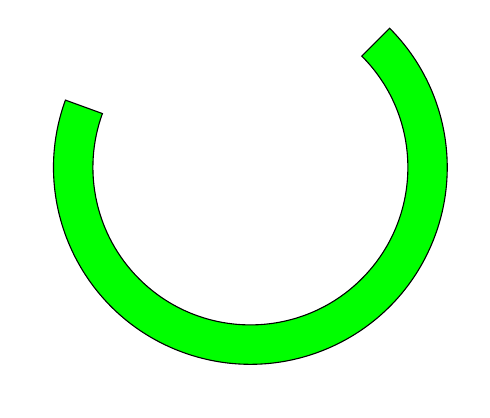
\begin{tikzpicture}
 
 \coordinate (c2) at (0,0);
   \draw[fill=green]
  % radius=5mm, initial=45, final=270
  ($(c2) + (45:20mm)$) arc (45:-200:20mm)
  --
  % radius=6mm, reversed
  ($(c2) + (-200:25mm)$) arc (-200:45:25mm)
  -- cycle;
\end{tikzpicture}
\fi

		\end{enumerate}
	\end{enumerate}
\end{enumerate}
\section{Rules of the air}
\begin{enumerate}
	\item When two airplanes are approaching head-on, each must alter direction. What direction?\hfill\textbf{Right}
	\item When overtaking another aircraft, who has the right of way?\hfill\mbox{\textbf{The overtaking aircraft}}
	\item Describe how to overtake a slower aircraft in front of you.\hfill\mbox{\textbf{Passing to the right}}
	\item Landing aircraft have right-of-way over aircraft taking off?\hfill\textbf{TRUE}
	\item When two aircraft are on converging headings, the aircraft on the right has right of way\hfill\textbf{FALSE}
	\item When operating at a non-controlled aerodrome, at what height AGL may we turn after take-off?\vfill\textbf{500\,ft}
	\item At a Class D aerodrome, if the previous aircraft is landing, it must be clear of the runway prior to you touching down.\hfill\textbf{TRUE}
	\item May we smoke in an airplane?\hfill\textbf{No.}
	\item Can we smoke whilst refuelling?\hfill\textbf{No if closer than 15\,m}
	\item Alcohol consumption. As per CAR 256/CASR99/MFT DAMP, the consumption of alcohol by flight crew is 
	prohibited for a period of at least how many hours prior to departure? What are some other drug and
	alcohol considerations?\hfill\textbf{8 hours}

\end{enumerate}
\section{Class D radio procedures}
\begin{enumerate}
	\item When contacting Moorabbin tower to report ready for circuits at 17L, what do we say?

	\textbf{Moorabbin Tower, <callsign>, for circuits, <dual/solo>, ready, 17L.}
	\item What is our downwind call for a touch and go?

	\textbf{<callsign>, turning downwind, touch-n-go.}
	\item What do we say when we are going around? Is it priority to advise the tower of this?
	
	\textbf{<callsign>, going around. Not a priority.}
	\item What are your actions if you lose sight of traffic you're following?

	\textbf{<callsign> traffic not sighted}
	\item Who provides traffic separation at Moorabbin?

	\textbf{Pilots and ATC}
	\item State the purpose of the following radio switches:
	\begin{enumerate}
		\item Avionics master: \textbf{Turn on all avionics and radios}
		\item Squelch control: \textbf{N/A}
		\item Transmit button: \textbf{Open mic for broadcast}
	\end{enumerate}
	\item Write examples of 
	\begin{enumerate}
		\item DISTRESS

		\textbf{MAYDAY MAYDAY MAYDAY, UNIFORM UNIFORM DELTA UNIFORM UNIFORM DELTA UNIFORM UNIFORM DELTA. 2 MILES TO THE SOUTH OF MOORABBIN, 1500 FT. ENGINE FAILURE. RETURNING TO THE AIRPORT}
		\item urgency \textbf{PAN-PAN PAN-PAN PAN-PAN, UUD UUD UUD. MID DOWNWIND MOORABBIN, 1000 FT. UNABLE TO DEPLOY FLAPS. INBOUND TO LAND.}
		\item Radio failure
		\begin{enumerate}
			\item Fly the plane.
			\item Squawk 7600.
			\item Continue transmitting, prefixing with TRANSMITTING BLIND.
			\item Monitor ATIS.
			\item Overfly at 1500\,ft. Observe traffic pattern. Enter circuit via crosswind.
			\item Look for instructions from the tower.
		\end{enumerate}
	\end{enumerate}
\end{enumerate}
\section{Emergencies}
\begin{enumerate}
	\item What do we do in case of engine fire at startup?
	\begin{enumerate}
		\item Release starter
		\item Close fuel selector
		\item Throttle idle
		\item Magnetos off
		\item Retain fire extinguisher.
		\item Harness off, hatches off, evacuate.
		\item Call 000
	\end{enumerate}
	\item Engine fire at cruise?
	\begin{enumerate}
		\item Heating off
		\item Fuel selector: off.
		\item Throttle: full
		\item Magnetos: once fuel consumed---off.
		\item Select landing area.
		\item Land ASAP.
		\item Evacuate.
	\end{enumerate}
	\item Engine failure in circuit:
	\begin{enumerate}
		\item Fly best glide speed (70\,KIAS). 
		\item Choose most suitable runway, aiming for 1/3 down the runway unless sure can reach field, taking into account wind.
		\item Declare mayday, communicate intentions.
		\item Land. Power to idle once landing field within range.
	\end{enumerate}
	\item Normal lift-off speed? \hfill\textbf{55\,KIAS}
	\item Best glide speed?\hfill\textbf{70\,KIAS}
\end{enumerate}
\section{Engine ice and handling}
\begin{enumerate}
	\item List some methods of keeping the engine within operating limits.

	\textbf{Avoid violent changes of power, especially after a steep descent. Do not exceed maximum RPM times. Use mixture control if available}
	\item What controls the fuel/air ratio being delivered to the airplane?

	\textbf{Mixture or throttle}
	\item Describe the method of applying full power on take-off.

	\textbf{Push forward over 4 seconds, applying right rudder. Monitor RPM, engine temps, airspeed}
	\item How do you level off to cruise?

	\textbf{Lower the nose. Wait for airspeed to increase. Reduce power to 4800\,RPM. Trim}
	\item Throttle on approach

	\textbf{Adjust power on base to control height; adjust power on final to control speed}
	\item Where are power setting, oil temperature, and EGT displayed in the cockpit. 

	\textbf{Main avionics panel}
\end{enumerate}
\section{Climbing}
\begin{enumerate}
	\item What is the best rate of climb (\(V_y\)) in the Sling 2?\hfill\textbf{72\,KIAS}
	\item What is the best angle of climb (\(V_x\)) speed?\hfill\textbf{65\,KIAS}
	\item When would we use the best rate of climb speed?\hfill\textbf{Takeoff leg; complying with ATC instruction}
	\item What would we use the best angle of climb?\hfill\textbf{Obstacle clearance}
	\item What effect does a headwind have on rate of climb?\hfill\textbf{None.}
\end{enumerate}
\section{Descending}
\begin{enumerate}
	\item What would happen to flight path if we decreased our power on descent yet held a constant airspeed?

	\textbf{Attitude would decrease}
	\item And if we lowered flap?

	\textbf{Attitude would decrease}
\end{enumerate}

\section{Lift and drag}
\begin{enumerate}
	\item Define the lift formula and then simplify it to the pilot's lift formula.
	\[L = C_L\times\frac{\rho}{2}V^2S \]
	\item Complete the following table:

	\begin{tabular}{lccc}
	\toprule
	& & \textbf{Lift} & \textbf{Total drag} \\
	\midrule
	\textbf{Airspeed} & \(\uparrow\)   & \(\uparrow\)   & \(\uparrow\) \\
	                  & \(\downarrow\) & \(\downarrow\) & \(\downarrow\) \\
	\textbf{AoA}      & \(\uparrow\)   & \(\uparrow\)   & \(\uparrow\)\\
	                  & \(\downarrow\) & \(\downarrow\) & \(\downarrow\) \\
  \textbf{FLAP}     & \(\uparrow\)   & \(\downarrow\) & \(\downarrow\) \\
                    & \(\downarrow\) & \(\uparrow\)   & \(\uparrow\) \\
  \bottomrule
	\end{tabular}
	\end{enumerate}
\section{Power}
When we increase power the slipstream effect will also increase.
\begin{enumerate}
	\item What if any flight controls will be affected?

	\textbf{Rudder}
	\item When we increase power our attitude will change. 

	\textbf{Pitch down}
	\item Why does control effectiveness improve with a higher IAS?

	\textbf{Control are determined by deflecting air}
\end{enumerate}


\end{document}


